\section{Experiments}
We conduct our main experiments to evaluate SliderSpace using SDXL-DMD~\cite{dmd}, a 4-step distilled diffusion model. Our implementation requires less than 24GB VRAM and can discover 64 semantic directions in under 2 hrs on a single A100 GPU. When concepts exhibit severe mode collapse, the discovery process can be enhanced by generating data using undistilled base models or LLM-expanded prompts for increased sample diversity. We demonstrate SliderSpace's generalization to SDXL~\cite{podell2023sdxl}, SDXL-Turbo~\cite{turbo}, and transformer-based FLUX Schnell~\cite{flux} in appendix. Our analysis focuses on three key applications: concept decomposition, art styles exploration, and diversity enhancement in distilled models.

% \section{Experiments}
% We conduct our main experiments to evaluate SliderSpace using SDXL-DMD~\cite{dmd}, a 4-step distilled diffusion model. We also demonstrate SliderSpace's generalization to SDXL~\cite{podell2023sdxl}, SDXL-Turbo~\cite{turbo}, and transformer-based FLUX Schnell~\cite{flux} in appendix. Our analysis focuses on three key applications: concept decomposition, art styles exploration, and diversity enhancement in distilled models.

\subsection{Concept Decomposition} \label{sec:concept_exp}
We first demonstrate how SliderSpace can serve as an exploratory tool by decomposing high-level concepts into semantic directions that align with the diffusion model's internal representations. Summarizing and exposing the dominant variations a model is capable of for a particular prompt.

Given a concept prompt (e.g., "picture of a monster"), we discover SliderSpace directions.Figure~\ref{fig:concept} shows discovered sliders for ``Monster'', and ``car'' concepts. We label the sliders using Claude 3.5 Sonnet~\cite{claude} by showing multiple image pairs showing the effect of each slider and prompting to identify the semantic transformation being applied. Through these discovered directions, we demonstrate the manipulation of individual attributes. As these directions are intended to capture the model's visual possibilities for a prompt, we naturally ask the question, \textit{``How much variation is enabled by these directions?''}. To quantitatively evaluate the diversity enabled by SliderSpace against base model, we compute DreamSim \cite{dreamsim} distance to measure inter-image variation across 2500 generated samples per concept  (Figure~\ref{fig:concept-diversity}). For SliderSpace-augmented generation, we generate the images by randomly activating a sparse subset of 3 sliders (out of 32 discovered directions) for each generation. Our analysis reveals that SliderSpace-generated samples exhibit significantly higher inter-image diversity compared to the baseline model outputs. We measure the CLIP-Score~\cite{hessel2021clipscore} between the input prompts and the generated images to measure text-alignment with the prompt. We find that they have similar CLIP Scores to the images generated by the base model. This suggests that SliderSpace effectively expands the achievable variation in the model's knowledge, while maintaining semantic consistency. To validate our findings through human perception, we conducted pairwise comparisons of image grids generated by SliderSpace versus baseline methods. As shown in Table~\ref{tab:userconcept}, users consistently preferred SliderSpace outputs across diversity, utility, and creative potential.

\begin{figure*}
    \centering
    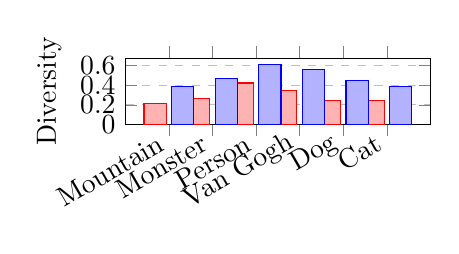
\begin{tikzpicture}[baseline, xshift=-0.3\textwidth]
    \begin{axis}[
            % Basic settings
            width=0.45\textwidth,
            height=0.2\textwidth,
            ylabel={Diversity},
            % Bar settings
            ybar=2pt,   % Gap between bars
            bar width=8pt,
            symbolic x coords={Mountain, Monster, Person, Van Gogh, Dog, Cat},
            xtick=data,
            enlarge x limits=0.2,
            % Legend settings
            legend image code/.code={%
                \draw[#1, draw=none] (0cm,0cm) rectangle (0.3cm,0.2cm);
            },
            legend style={
                at={(0.9,-0.05)},  % Position in upper right
                anchor=north west,  % Anchor point
                draw=none,         % No border
                fill=none,         % No background
                legend columns=1
            },
            % Y-axis settings
            ymin=0,
            ymajorgrids=true,
            grid style=dashed,
            % Rotated x labels
            x tick label style={
                rotate=30,
                anchor=east
            },        ]
        % Baseline method
        \addplot[red,fill=red!30] coordinates {
            (Mountain,0.217)
            (Monster,0.266)
            (Person,0.423)
            (Van Gogh,0.349)
            (Dog,0.246)
            (Cat,0.246)        };

        
        % Our method
        \addplot[blue,fill=blue!30] coordinates {
            (Mountain,0.387)
            (Monster,0.472)
            (Person,0.613)
            (Van Gogh,0.557)
            (Dog,0.444)
            (Cat,0.387)        };
        
        \end{axis}
    \end{tikzpicture}
    \hspace{0.02\textwidth}
    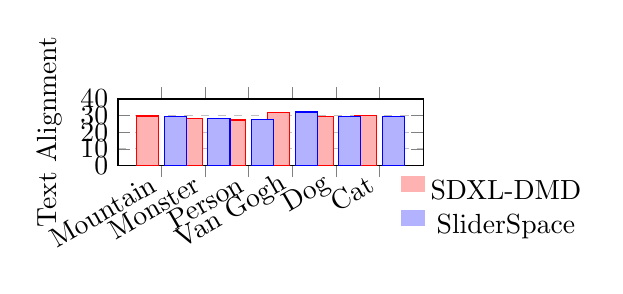
\begin{tikzpicture}[baseline, xshift=0.3\textwidth]
    \begin{axis}[
            % Basic settings
            width=0.45\textwidth,
            height=0.2\textwidth,
            ylabel={Text Alignment},
            % Bar settings
            ybar=2pt,   % Gap between bars
            bar width=8pt,
            symbolic x coords={Mountain, Monster, Person, Van Gogh, Dog, Cat},
            xtick=data,
            enlarge x limits=0.2,
            % Legend settings
            legend image code/.code={%
                \draw[#1, draw=none] (0cm,0cm) rectangle (0.3cm,0.2cm);
            },
            legend style={
                at={(0.9,-0.05)},  % Position in upper right
                anchor=north west,  % Anchor point
                draw=none,         % No border
                fill=none,         % No background
                legend columns=1
            },
            % Y-axis range
            ymin=0,
            ymax=40.0,  % Set maximum y value
            % Y-axis settings
            ymin=0,
            ymajorgrids=true,
            grid style=dashed,
            % Rotated x labels
            x tick label style={
                rotate=30,
                anchor=east
            },        ]
        % Baseline method
        \addplot[red,fill=red!30] coordinates {
            (Mountain,29.75)
            (Monster,28.14)
            (Person,27.38)
            (Van Gogh,31.94)
            (Dog,29.38)
            (Cat,29.95)        };

        
        % Our method
        \addplot[blue,fill=blue!30] coordinates {
            (Mountain,29.33)
            (Monster,28.14)
            (Person,27.40)
            (Van Gogh,32.20)
            (Dog,29.20)
            (Cat,29.20)        };
        
        \legend{SDXL-DMD, SliderSpace}
                
        \end{axis}
    \end{tikzpicture}    \caption{(left) SliderSpace generates diverse variations of a concept, as measured by DreamSim~\cite{dreamsim} distance across generated samples (higher is better). (right) The method maintains similar text-to-image alignment, as measured by CLIP Scores~\cite{hessel2021clipscore} (lower is better). }
    \label{fig:concept-diversity}
\end{figure*}

\begin{table}
    \centering
    \small
    \begin{tabular}{rccc}
         & \multicolumn{3}{c}{\textbf{User Study (Win Rate \%)}} \\
        \textbf{Method vs.} & \textbf{``Diverse''} & \textbf{``Useful''}  & \textbf{``Creative''} \\
        \hline
        SDXL-DMD &  72.4 & 66.0 & 68.1 \\
        LLM + SDXL-DMD & 62.5 & 62.5 & 62.5 \\
        SDXL & 65.3 & 61.2 & 59.2  \\

    \end{tabular}
    \caption{Users perceive SliderSpace generated images to be more diverse, useful, and interesting. We show win-rate percentages of SliderSpace samples against baselines.}
    \label{tab:userconcept}
\end{table}
%\begin{table}
    \centering
   \begin{tabular}{lcccc}
        % \hline
        & \multicolumn{2}{c}{\textbf{Base Model}} & \multicolumn{2}{c}{\textbf{SliderSpace}} \\
        \textbf{Concept} & \textbf{Diversity} & \textbf{CLIP} & \textbf{Diversity} & \textbf{CLIP} \\
        \hline
        Monster & 0.266  & 28.14 & 0.472  & 28.37 \\
        Mountain & 0.217  & 29.75 & 0.387  & 29.33 \\
        Person & 0.423 & 27.38 & 0.613 & 27.40 \\
        Van Gogh & 0.349  & 31.94 & 0.557  & 32.20 \\
        Cat & 0.145  & 29.95 & 0.387  & 30.20 \\
        Dog & 0.246  & 29.38 & 0.444 & 29.20 \\

    \end{tabular}
    \caption{SliderSpace enables diverse image generation as indicated by DreamSim\cite{dreamsim} distance across generated images while also having a good text-to-image alignment through CLIP scores. [Diversity - can be thought as a way to measure model's recall of diverse visual variations; CLIP - can be thought as measuring precision of the model's output by evaluating how relevant the images are to the prompt used.]}
    \label{tab:dreamsim}
\end{table}

\subsection{Art Styles Exploration} \label{sec:art_exp}
We also evaluate to what degree SliderSpace can expose ``all'' of the art styles that the diffusion model has learned from its training data. As a proxy for ``all'', we use a diverse set of art styles, manually discovered and documented by ParrotZone~\cite{parrotzone}. We explore the visual artistic space by decomposing the prompt ``artwork in the style of a famous artist'' into 64 directions. This process enables us to discover the SliderSpace of art and create a comprehensive dictionary of discoverable art styles in a diffusion model.

To compare how this measures up against supervised methods like Concept Slider~\cite{gandikota2023concept}, we train 64 manually curated concept sliders using LLM generated training prompts. We compute FID scores against the generated samples conditioned on actual artist names from ParrotZone~\cite{parrotzone} dataset. The dataset contains 4388 artists mimicked by SDXL, are discovered through exhaustive manual search. We also establish two other baselines. First, we use GPT/Claude to generate 4388 different artistic style names (e.g., ``cubism'', ``Warhol''). Second, we use a generic prompt like ``[subject] in the style of a famous artist''. Using our discovered SliderSpace, we randomly sample a sparse set of 3 sliders to generate an equivalent number of images. Specifically, for each baseline, we match the provided samples of \cite{parrotzone} by creating two images per style for ``building landscape'' and ``character portraits'' each (total of four images per style) to ensure same semantic structure across the datasets and that FID measures the artistic spread. Figure~\ref{fig:artcompare} shows random, non-cherry picked images from all the methods and their corresponding FID scores. We find that SliderSpace generates a distribution significantly more closely matches the manually curated artist names than the baselines, including supervised methods like Concept Sliders. Figure~\ref{fig:artqualitative} shows qualitative comparison of art styles discovered by SliderSpace and styles discovered manually ~\cite{parrotzone}.
\begin{figure*}
    \centering
    \includegraphics[width=\linewidth]{figures-src/art_comparison.pdf}
    \caption{SliderSpace demonstrates broader artistic style coverage, as evidenced by the lower FID scores compared to both supervised Concept Sliders. Comparison of artistic style diversity using FID scores against reference distribution (a) derived from the complete artist dataset~\cite{parrotzone}. We compare against outputs from (b) generic art prompts (b), (c) LLM-generated art prompts, and (d) Concept Sliders.}
    \label{fig:artcompare}
\end{figure*}


\begin{figure*}[htbp]
    \centering
    \includegraphics[width=\linewidth]{figures-src/art-real_sliderspace_final.pdf}
    \caption{Comparison of artistic styles discovered in SDXL-DMD: (Left) Representative samples from artist-specific prompts manually curated by the Parrotzone community~\cite{parrotzone} through extensive exploration. (Right) Automatically discovered artistic directions using SliderSpace, which captures diverse and semantically meaningful variations without requiring explicit artist references.}
    \label{fig:artqualitative}
\end{figure*}

To validate the practical utility of our ``artistic'' SliderSpace, we conduct a user study examining both usefulness and diversity of generated samples (Table~\ref{tab:userart}). We conduct comparitive study with 2 grids of 9 images (total of 1000 pairs), one with slider generated images and other with baselines. Users find the SliderSpace-generated images are far more diverse and useful than the baseline methods. We also find that users would prefer using SliderSpace images over images prompted with the real artist names~\cite{parrotzone}, while finding these both to be equally diverse. We provide more userstudy details and qualitative examples in Appendix.

\begin{table}
    \centering
    \small
    \begin{tabular}{rcc}
       & \multicolumn{2}{c}{\textbf{User study (win rate \%)}} \\
        \textbf{Method} & \textbf{``Diverse''} & \textbf{``Useful''}  \\
        \hline
        \,vs.\, Real Artist Prompts~\cite{parrotzone} &  54 & 63  \\
        \,vs.\, LLM Prompts & 73 & 67 \\
        \,vs.\, Generic Prompts & 87 & 88   \\

    \end{tabular}
    \caption{Pairwise comparison user study (win rates in \%) reveals that SliderSpace-extracted artistic styles achieve comparable diversity to manually curated artist~\cite{parrotzone}, while being significantly preferred for creative utilization. 
    % Our approach effectively discovers latent artistic capabilities without requiring manual identification of artist names in the model.
    }
    \label{tab:userart}
\end{table}


\subsection{Diversity Enhancement} \label{sec:diverse_exp}
Finally, we explore SliderSpace's ability to addressing mode collapse in distilled models. Instead of discovering SliderSpace for narrow distributions, we train it on a larger spread of 8000 randomly selected COCO-30k prompts and enhance them with LLM. We use DMD model for generating training dataset since we wish to undo mode collapse of DMD models. We discover a generic SliderSpace of 64 sliders that captures the generally applicable visual variations within SDXL-DMD. Figure ~\ref{fig:diverse} showcases qualitative examples of two distributions for the prompts ``Car driving through a forest'' and ``Picture of a person''. We demonstrate how generating images by randomly sampling from these SliderSpace directions effectively increases output diversity. This demonstrates that the mode collapse in distilled model can be reversed by discovering and exploring the visual structure. We show more examples in appendix.
\begin{figure*}
    \centering
    \includegraphics[width=.95\linewidth]{figures-src/diverse.pdf}
    \caption{SliderSpace can also decompose general broad visual variation of diffusion model's and can be used to overcome model collapse in distilled models. We randomly sample a sparse set of sliders and generate the sample showing higher variation than base distilled model.}
    \label{fig:diverse}
\end{figure*}


In Table~\ref{tab:diverse}, we evaluate this improvement by measuring FID and CLIP scores on all COCO-30k prompts before and after applying SliderSpace to SDXL-DMD. We find that DMD-SliderSpace improves FID from the distilled version, almost matching the FID of undistilled SDXL. 
% \begin{table*}[h!]
% \centering
% \small
% \begin{tabular}{lccccc}
% \toprule
% \textbf{Diversity} & \textbf{FigureQA} & \textbf{DVQA} & \textbf{PlotQA} & \textbf{ChartQA} & \cellcolor[gray]{0.9}\textbf{Ours (Charts)} \\
% \midrule
% Image & 0.268 & 0.307 & 0.420 & 0.340 & \cellcolor[gray]{0.9}\textbf{0.596} \\
% Text & 0.567 & 0.752 & 0.743 & 0.742 & \cellcolor[gray]{0.9}\textbf{0.823} \\
% \bottomrule
% \end{tabular}
% \vspace{-.1cm}
% \caption{\textbf{Comparison of image and text diversity across different chart datasets.} We randomly sample 10K instances from each dataset to calculate the results.}
% \label{tab:diversity}
% \vspace{-.3cm}
% \end{table*}

\begin{table}[H]
\centering
\small
\begin{tabular}{lcc}
\toprule
\textbf{Dataset} & \textbf{Image Diversity} & \textbf{Text Diversity} \\
\midrule
FigureQA & 0.268 & 0.567 \\
DVQA & 0.307 & 0.752 \\
PlotQA & 0.420 & 0.743 \\
ChartQA & 0.340 & 0.742 \\
\cellcolor[gray]{0.9}Ours (Charts) & \cellcolor[gray]{0.9}\textbf{0.596} & \cellcolor[gray]{0.9}\textbf{0.823} \\
\bottomrule
\end{tabular}
\vspace{-.1cm}
\caption{\textbf{Compare image and text diversity across different chart datasets.} We randomly sample 10K instances from each dataset to compute the results.}
\label{tab:diversity}
\vspace{-.1cm}
\end{table}


\subsection{Slider Transferability}
Using FaceNet~\cite{schroff2015facenet} as the semantic encoder, we train SliderSpace on the concept ``person'' and discover interpretable directions controlling attributes like appearance and age (Figure~\ref{fig:transfer}). These directions not only transfer effectively to related concepts like ``police'' and ``athlete'' but also generalize surprisingly well to out-of-domain concepts like ``dog'', suggesting that SliderSpace captures fundamental visual transformations in the model's knowledge space.
% A key advantage of SliderSpace is the transferability of discovered directions across related concepts. We train SliderSpace on the general concept ``person'', in Figure~\ref{fig:transfer}, using FaceNet model~\cite{schroff2015facenet} as semantic encoder to extract PCA directions. We discover interpretable semantic directions controlling various attributes like appearance, accessories, age, and expressions. These learned directions successfully transfer to related concepts like ``police'' and ``athlete'' without additional training, enabling efficient slider reuse across related domains. Surprisingly, many sliders demonstrate transferability even to out-of-domain concepts. For instance, directions discovered for ``person'' can meaningfully modify attributes of generated ``dog'' images, suggesting that SliderSpace captures fundamental visual transformations that generalize across concepts.

\begin{figure*}[!ht]
    \centering
    \includegraphics[width=.95\linewidth]{figures-src/transfer.pdf}
    \caption{SliderSpace directions for the ``person'' concept successfully generalize to related ``police'' and ``athlete'' concepts. They also transfer to out-of-domain concepts like ``dog''}
    \label{fig:transfer}
\end{figure*}

Additional experiments analyzing hyperparameter choices (App.~\ref{sec:hyperparam}), alternative semantic embeddings (App.~\ref{sec:semantic}), and ablation studies (App.~\ref{sec:ablations}) are in Appendix.